\documentclass{template/openetcs_article}
% Use the option "nocc" if the document is not licensed under Creative Commons
%\documentclass[nocc]{template/openetcs_article}
\usepackage {bsymb,b2latex}
\usepackage{lipsum,url,color}
\graphicspath{{./template/}{.}{./images/}}
\begin{document}
\frontmatter
\project{openETCS}

%Please do not change anything above this line
%============================
% The document metadata is defined below

%assign a report number here
\reportnum{OETCS}

%define your workpackage here
\wp{Work-Package 7: ``Toolchain''}


\newcommand{\true}{\ensuremath{true}}
\newcommand{\btext}[1]{{\it #1}}
\newcommand{\bvar}[1]{\btext{#1}}
\newcommand{\bevent}[1]{\btext{#1}}
\newcommand{\binv}[1]{\btext{#1}}
\newcommand{\bconst}[1]{\btext{#1}}
\newcommand{\bparam}[1]{\btext{#1}}
\newcommand{\bfunc}[1]{\btext{#1}}
\newcommand{\baxiom}[1]{\btext{#1}}
\newcommand{\btype}[1]{\btext{#1}}
\newcommand{\bguard}[1]{\btext{#1}}
\newcommand{\bmachine}[1]{\btext{#1}}
\newcommand{\bctx}[1]{\btext{#1}}

\author{Matthias Güdemann\\Systerel, France}

\affiliation{Systerel}

\title{Event-B Model of Subset 026, Section 4.6}

% define the coverart
\coverart[width=350pt]{chart}

\reporttype{Model Description}

%\begin{document}

\maketitle
\tableofcontents
\listoffiguresandtables
\newpage

This document describes a formal model of the requirements of section~4.6 of the
subset 026 of the ETCS specification 3.3.0~\cite{ETCS}. This section describes
the transition table between the different train modes. This includes the
transition conditions and their respective priorities.

The model is expressed in the formal language Event-B~\cite{eventB} and
developed within the Rodin tool~\cite{rodin}. This formalism allows an iterative
modeling approach. In general, one starts with a very abstract description of
the basic functionality and step-wise adds additional details until the desired
level of accuracy of the model is reached. Rodin provides the necessary proof
support to ensure the correctness of the refined behavior.

In this document we present an Event-B model of the transitions from stand-by to
shunting, from stand-by to full supervision and from stand-by to isolation. The
transition table is expressed as a graphical model of a state machine which is
automatically translated into Event-B code.


\begin{table}[ht]
  \centering
  \begin{tabular}[ht]{|l|l|}
    \hline
    SB & stand-by \\
    \hline
    FS & full supervision \\
    \hline
    IS & isolation \\
    \hline
    SH & shunting \\
    \hline
    MA & movement authority \\
    \hline
    SRS & system requirements specification \\
    \hline
  \end{tabular}
  \caption{Glossary}
  \label{tab:glossary}
\end{table}

\section{Short Introduction to Event-B}
\label{sec:short-intr-event}

The formal language Event-B is based on a set-theoretic approach. It is a
variant of the B language, with a focus on system level
modeling~\cite{eventbbook}. An Event-B model is separated into a static and a
dynamic part.

The dynamic part of an Event-B model describes abstract state machines. The
state is represented by a set of state variables. A transition from one state to
another is represented by parametrized events which assign new values to the
state variables. Event-B allows unbounded state spaces. They are constrained by
invariants expressed in first order logic with equality which must be fulfilled
in any case. The initial state is created by a special initialization event.

The static part of an Event-B model is represented by contexts. These consist of
carrier sets, constants and axioms. The type system of a model is described by
means of carrier sets and constraints expressed by axioms.

Event-B is not only comprised of descriptions of abstract state machines and
contexts, but also includes a development approach. This approach consists of
iterative refinement of the machines until the desired level of detail is
reached. In the Rodin tool, proof obligations are automatically created which
ensure correct refinement.

Together with the machine invariants, the proof obligations for the refinement
are formally proven, creating proof trees. To accomplish this, there are
different options: many proof obligations can be discharged by automated provers
(e.g., AtelierB, NewPP, Rodin's SMT-plugin), but as the underlying logic is in
general undecidable, it is sometimes necessary to use the interactive proof
support of Rodin.

Any external actions, e.g., mode changes by the driver or train level changes
are modeled via parametrized events. Only events can modify the variables of a
machine. An Event-B model is on the system level, events are assumed to be
called from a software system into which the functional model is embedded. The
guards of the events assure that any event can only be called when appropriate.

\section{Modeling Strategy}
\label{sec:modeling-strategy}

The description of the section~4.6. of the SRS consists of a large table which
describes the possible transitions from one mode to another and the necessary
preconditions of a transition. The table also specifies different priorities and
the relative priorities of the transitions, i.e., to ensure an explicit
precedence if more than one condition is enabled.

The model view consists of a state machine representing the current state,
external events can trigger the prerequisites for the conditions. Priorities are
modeled by negating a condition with a higher priority for a conditions with a
lower priority. For example, let $q$ and $p$ be preconditions that can be
fulfilled at the same time, $q$ for event \bevent{evt\_q} and $p$ for event
\bevent{evt\_p}. Let $q$ have a higher priority than $p$. In Event-B this
precedence can be modeled by using $q$ as condition for \bevent{evt\_q}, and
$\neg q \wedge p$ for $evt_p$, i.e., the preconditions for the two events cannot
be fulfilled at the same time.

The state machine itself is modeled using the iUML statemachine
plugin~\footnote{\url{http://wiki.event-b.org/index.php/Event-B_Statemachines}}
which allows graphical modeling of state machines. The model start with the
basic possibilities for the transitions between the modes. The conditions are
iteratively refined and external events added to the model.

\section{Model Overview}
\label{sec:model-overview}

Figure~\ref{fig:model-overview} shows the model overview. The left column shows
the different state machines and the right column the context. An arrow from one
machine to another represents a refinement relation, an arrow from a machine to
a context represents a sees relation.

\begin{figure}[ht]
  \centering
  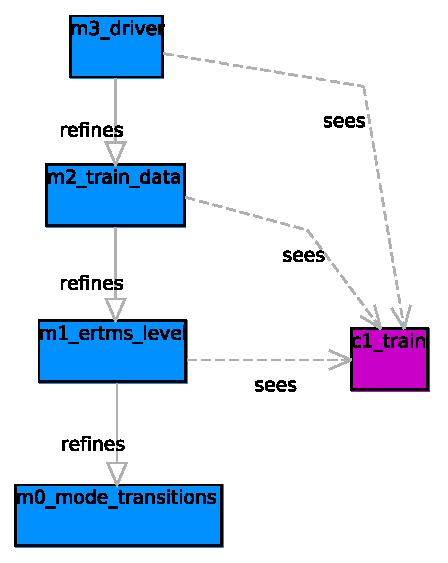
\includegraphics[width=.35\textwidth]{Subset_026_Chap_4_6}
  \caption{Machine Refinements and Contexts}
  \label{fig:model-overview}
\end{figure}

The model starts with the principal possibilities for the transitions from mode
SB to FS, SB to IS and SB to SH. This is realized in the machine $m0$. The
refinement in $m1$ implements the dependency on the train behavior and ETCS
levels which are introduced in the context $c1$. The refined machine $m2$ allows
for storing abstract train data and gradient information for a movement
authority. The refinement in $m3$ finally introduces the external driver who can
trigger events.

\section{Model Benefits}
\label{sec:model-highlights}

The Event-B model in Rodin has some interesting properties which are highlighted
here. Some stem from the fact that Rodin is well integrated into the Eclipse
platform which renders many useful plugins available, both those explicitly
developed for integration with Rodin, but also other without Rodin in mind.
Other interesting properties stem from the fact that Rodin and Event-B provide
an extensive proof support for properties.

\begin{itemize}
\item {\bf Refinement} The Event-B approach allows iterative development based
  on refinement. This allows starting modeling with a very abstract machine and
  then step-wise adding more detailed behavior. Rodin generates all the
  necessary proof obligations which are required to assure correct refinement.
\item {\bf Requirements Tracing} Rodin provides an extensible EMF model,
  therefore it is easily possible to trace requirements using the requirements
  modeling framework of Eclipse (RMF) via the ProR plugin. This allows the usage
  of requirement documents in the OMG standardized Requirements Interchange
  Format (ReqIF).
\item {\bf Model Animation} The Event-B model can be animated via different
  plugins, e.g., ProB or AnimB. This allows the simulation of the model, by
  clicking on the activated events and tracking the resulting state of the
  variables. This technique allows to examine the run-time behavior of the
  model, e.g., for testing purposes. There is also ongoing development for a
  model-based testing plugin in Rodin, which will allow storing and replaying of
  event sequences.
\item {\bf Graphical Modeling} Rodin supports graphical modeling via its plugin
  mechanism. The iUML statemachine plugin allows for graphical state machine
  modeling and animation via ProB. The graphical model is automatically
  translated into the Event-B language.
\end{itemize}

\section{Detailed Model Description}
\label{sec:deta-model-descr}

This section describes the formal model in more detail. For each refinement the
new state variables are introduced and their meaning is explained. The machines
are not fully presented, only the relevant changes done in the refinement.

The modes and transitions between  the modes are modeled graphically using the
iUML statemachine plugin. In this notation, transitions are labeled with events,
i.e., the transitions are active if the preconditions of the respective events
are fulfilled.

In the graphical model, it is possible to have multiple events triggering a
transition, the semantics of this is the disjunction of the conditions, i.e.,
any single event can trigger the transition.

\subsection{Machine 0 - Mode Transitions}
\label{sec:machine-0-mode}

The first machine $m0$ implements the transition possibilities for the states
\bvar{SB}, \bvar{SH}, \bvar{FS} and \bvar{IS}. It is shown in
Figure~\ref{fig:statemachine-m0}. The transition labels represent events of the
Event-B machine. The initial state is \bvar{SB}, this is represented by the
\bevent{INITIALISATION} event from the UML initial state.

\begin{figure}[ht]
  \centering
  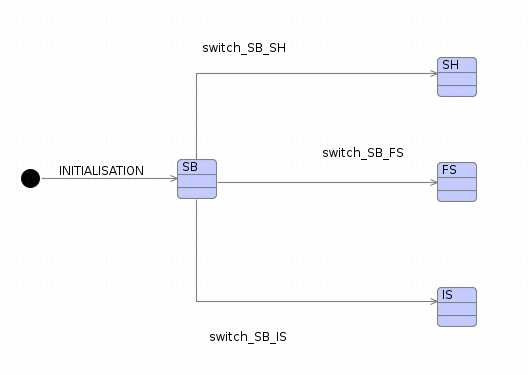
\includegraphics[width=.75\textwidth]{statechart1}
  \caption{Statemachine for Machine 0}
  \label{fig:statemachine-m0}
\end{figure}

The state machine is translated into Event-B code. Every state is represented as
a Boolean variable. An invariant ensures that there is always only a single
variable with the value ``TRUE'', i.e., the state machine is always in exactly
one state.

A transition will use these Boolean variables to analyze whether its source
state is active. A state change is encoded by changing the values of the
variables corresponding to the source and target state of the transition. For
more details on the possible encoding
see~\footnote{\url{http://wiki.event-b.org/index.php/Event-B_Statemachines}}.

\paragraph{Implemented Requirements}
\label{sec:impl-requ}

\begin{itemize}
\item §4.6.2 transition from \bvar{SB} to \bvar{SH}
\item §4.6.2 transition from \bvar{SB} to \bvar{FS}
\item §4.6.2 transition from \bvar{SB} to \bvar{IS}
\end{itemize}

\begin{description}
\VARIABLES
        \begin{description}
                \Item{ SB }
                \Item{ SH }
                \Item{ FS }
                \Item{ IS }
        \end{description}
\INVARIANTS
        \begin{description}
                \nItem{ typeof\_SB }{ SB \in  BOOL }
                \nItem{ typeof\_SH }{ SH \in  BOOL }
                \nItem{ typeof\_FS }{ FS \in  BOOL }
                \nItem{ typeof\_IS }{ IS \in  BOOL }
                \nItem{ distinct\_states\_in\_mode\_changes1 }{ partition(\{ TRUE\} , \{ SB\}  \binter  \{ TRUE\} , \{ SH\}  \binter  \{ TRUE\} , \{ FS\}  \binter  \{ TRUE\} , \{ IS\}  \binter  \{ TRUE\} ) }
        \end{description}
\EVENTS
        \INITIALISATION
                \begin{description}
                \BeginAct
                        \begin{description}
                        \nItem{ init\_IS }{ IS :=  FALSE }
                        \nItem{ init\_SB }{ SB :=  TRUE }
                        \nItem{ init\_SH }{ SH :=  FALSE }
                        \nItem{ init\_FS }{ FS :=  FALSE }
                        \end{description}
                \EndAct
                \end{description}
        \EVT {switch\_SB\_SH}
                \begin{description}
                \WhenGrd
                        \begin{description}
                        \nItem{ isin\_SB }{ SB = TRUE }
                        \end{description}
                \ThenAct
                        \begin{description}
                        \nItem{ enter\_SH }{ SH :=  TRUE }
                        \nItem{ leave\_SB }{ SB :=  FALSE }
                        \end{description}
                \EndAct
                \end{description}
        \EVT {switch\_SB\_FS}
                \begin{description}
                \WhenGrd
                        \begin{description}
                        \nItem{ isin\_SB }{ SB = TRUE }
                        \end{description}
                \ThenAct
                        \begin{description}
                        \nItem{ enter\_FS }{ FS :=  TRUE }
                        \nItem{ leave\_SB }{ SB :=  FALSE }
                        \end{description}
                \EndAct
                \end{description}
        \EVT {switch\_SB\_IS}
                \begin{description}
                \WhenGrd
                        \begin{description}
                        \nItem{ isin\_SB }{ SB = TRUE }
                        \end{description}
                \ThenAct
                        \begin{description}
                        \nItem{ enter\_IS }{ IS :=  TRUE }
                        \nItem{ leave\_SB }{ SB :=  FALSE }
                        \end{description}
                \EndAct
                \end{description}
\END
\end{description}


\subsection{Context 1 - Train}
\label{sec:context-1-train}

The first context introduces the notion of the different ETCS levels. It also
introduces a very abstract notion of the behavior of a train, either moving or
at standstill. At this model level, more detailed information is not necessary.

\begin{description}
\SETS
        \begin{description}
                \Item{ train\_behavior }
                \Item{ ERTMS\_level }
        \end{description}
\CONSTANTS
        \begin{description}
                \Item{ L0 }
                \Item{ L1 }
                \Item{ L2 }
                \Item{ L3 }
                \Item{ NTC }
                \Item{ standstill }
                \Item{ moving }
        \end{description}
\AXIOMS
        \begin{description}
                \nItem{ axm1 }{ partition(train\_behavior,\{ standstill\} ,\{ moving\} ) }		\nItem{ axm2 }{ partition(ERTMS\_level, \{ NTC, L0, L1, L2, L3\} ) }	\end{description}
\END
\end{description}


\subsection{Machine 1 - ERTMS Level}
\label{sec:machine-1-ertms}

The first refined machine uses the ETCS levels with the state variable
\bvar{current\_level} and the current train behavior with the state variable
\bvar{current\_behavior}. The ETCS level \bconst{NTC} is the initial level and
the initial behavior is \bconst{standstill}. These variables are modified by
their corresponding \bevent{change\_}-events.

\begin{figure}[ht]
  \centering
  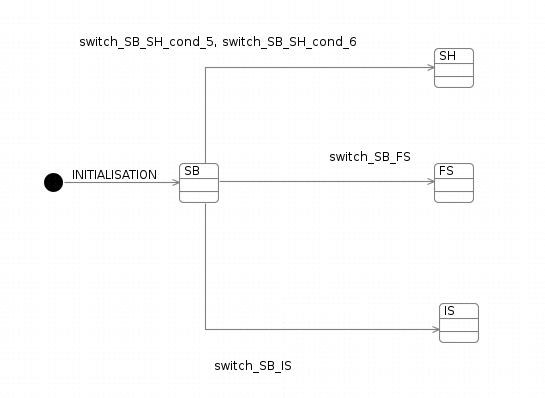
\includegraphics[width=.75\textwidth]{statechart2}
  \caption{Statemachine for Machine 1}
  \label{fig:statemachine-m1}
\end{figure}

The level and the behavior are used to refine the transition from \bvar{SB} to
\bvar{SH} into two different cases, dependent on the current ETCS level. This is
shown in the transition label in Figure~\ref{fig:statemachine-m1}.

\begin{description}
\REFINES{m0\_mode\_transitions}
\SEES{c1\_train}
\VARIABLES
        \begin{description}
                \Item{ current\_level }
                \Item{ current\_behavior }
        \end{description}
\INVARIANTS
        \begin{description}
                \nItemY{ inv1 }{ current\_level \in  ERTMS\_level }{  }
                \nItem{ inv2 }{ current\_behavior \in  train\_behavior }
        \end{description}
\EVENTS
        \INITIALISATION
                \\\textit{extended}
                \begin{description}
                \BeginAct
                        \begin{description}
                        \nItemY{ act1 }{ current\_level :=  NTC }{  }
                        \nItem{ act2 }{ current\_behavior :=  standstill }
                        \end{description}
                \EndAct
                \end{description}
        \EVT {change\_level}
                \begin{description}
                \AnyPrm
                        \begin{description}
                        \Item{l\_level }
                        \end{description}
                \WhereGrd
                        \begin{description}
                        \nItem{ grd1 }{ l\_level \in  ERTMS\_level }
                        \end{description}
                \ThenAct
                        \begin{description}
                        \nItem{ act1 }{ current\_level :=  l\_level }
                        \end{description}
                \EndAct
                \end{description}
        \EVT {change\_behavior}
                \begin{description}
                \AnyPrm
                        \begin{description}
                        \Item{l\_behavior }
                        \end{description}
                \WhereGrd
                        \begin{description}
                        \nItem{ grd1 }{ l\_behavior \in  train\_behavior }
                        \end{description}
                \ThenAct
                        \begin{description}
                        \nItemY{ act1 }{ current\_behavior :=  l\_behavior }{  }
                        \end{description}
                \EndAct
                \end{description}
        \EVT {switch\_SB\_SH\_cond\_5}
        \EXTD {switch\_SB\_SH}
                \begin{description}
                \WhenGrd
                        \begin{description}
                        \nItemX{ isin\_SB }{ SB = TRUE }
                        \nItem{ grd2 }{ current\_level \in  \{ NTC, L0, L1\}  }
                        \nItemY{ grd1 }{ current\_behavior = standstill }{ }
                        \end{description}
                \ThenAct
                        \begin{description}
                        \nItemX{ enter\_SH }{ SH :=  TRUE }
                        \nItemX{ leave\_SB }{ SB :=  FALSE }
                        \end{description}
                \EndAct
                \end{description}
        \EVT {switch\_SB\_SH\_cond\_6}
        \EXTD {switch\_SB\_SH}
                \begin{description}
                \WhenGrd
                        \begin{description}
                        \nItemX{ isin\_SB }{ SB = TRUE }
                        \nItemY{ grd1 }{ current\_behavior = standstill }{ }
                        \nItem{ grd2 }{ current\_level \in  \{ L2, L3\}  }
                        \end{description}
                \ThenAct
                        \begin{description}
                        \nItemX{ enter\_SH }{ SH :=  TRUE }
                        \nItemX{ leave\_SB }{ SB :=  FALSE }
                        \end{description}
                \EndAct
                \end{description}
\END
\end{description}


\subsection{Machine 2 - Train Data}
\label{sec:machine-2-train}

The second machine refinement adds the notion of valid train data and movement
authority gradient data. The validity of these two different kinds of data is
represented by the Boolean variables \bvar{valid\_train\_data} and
\bvar{MA\_SSP\_gradient\_data}. Both variables can be modified by two events;
one that stores valid data and one that deletes, i.e., invalidates the stored
data.

% \begin{figure}[ht]
%   \centering
%   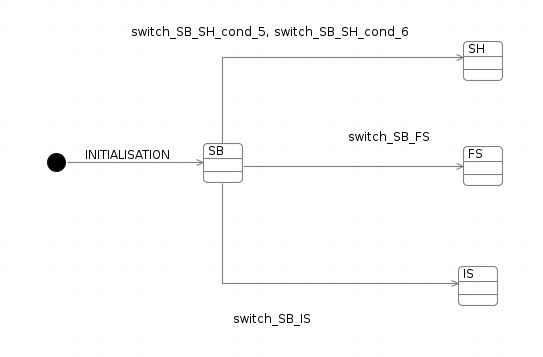
\includegraphics[width=.75\textwidth]{statechart3}
%   \caption{Statemachine for Machine 2}
%   \label{fig:statemachine-m2}
% \end{figure}

Having valid MA and train data is the precondition for the transition from
\bvar{SB} to \bvar{FS}. This transition is refined by guard strengthening.

\begin{description}
\REFINES{m1\_ertms\_level}
\SEES{c1\_train}
\VARIABLES
        \begin{description}
                \Item{ valid\_train\_data }
                \ItemY{ MA\_SSP\_gradient\_data }{}
        \end{description}
\INVARIANTS
        \begin{description}
                \nItem{ inv1 }{ valid\_train\_data \in  BOOL }
                \nItemY{ inv2 }{ MA\_SSP\_gradient\_data \in  BOOL }{  }
        \end{description}
\EVENTS
        \EVT {store\_valid\_train\_data}
                \begin{description}
                \WhenGrd
                        \begin{description}
                        \nItem{ grd1 }{ valid\_train\_data = FALSE }
                        \end{description}
                \ThenAct
                        \begin{description}
                        \nItem{ act1 }{ valid\_train\_data :=  TRUE }
                        \end{description}
                \EndAct
                \end{description}
        \EVT {remove\_valid\_train\_data}
                \begin{description}
                \WhenGrd
                        \begin{description}
                        \nItem{ grd1 }{ valid\_train\_data = TRUE }
                        \end{description}
                \ThenAct
                        \begin{description}
                        \nItem{ act1 }{ valid\_train\_data :=  FALSE }
                        \end{description}
                \EndAct
                \end{description}
        \EVT {store\_MA\_SSP\_gradient\_data}
                \begin{description}
                \WhenGrd
                        \begin{description}
                        \nItem{ grd1 }{ MA\_SSP\_gradient\_data = FALSE }
                        \end{description}
                \ThenAct
                        \begin{description}
                        \nItem{ act1 }{ MA\_SSP\_gradient\_data :=  TRUE }
                        \end{description}
                \EndAct
                \end{description}
        \EVT {remove\_MA\_SSP\_gradient\_data}
                \begin{description}
                \WhenGrd
                        \begin{description}
                        \nItem{ grd1 }{ MA\_SSP\_gradient\_data = TRUE }
                        \end{description}
                \ThenAct
                        \begin{description}
                        \nItem{ act1 }{ MA\_SSP\_gradient\_data :=  FALSE }
                        \end{description}
                \EndAct
                \end{description}
        \EXTD {switch\_SB\_FS}
                \begin{description}
                \WhenGrd
                        \begin{description}
                        \nItemX{ isin\_SB }{ SB = TRUE }
                        \nItemY{ grd1 }{ MA\_SSP\_gradient\_data = TRUE }{ }
                        \nItem{ grd2 }{ valid\_train\_data = TRUE }
                        \end{description}
                \ThenAct
                        \begin{description}
                        \nItemX{ enter\_FS }{ FS :=  TRUE }
                        \nItemX{ leave\_SB }{ SB :=  FALSE }
                        \end{description}
                \EndAct
                \end{description}
\END
\end{description}


\subsection{Machine 3 - Driver}
\label{sec:machine-3-driver}

The next machine refinement adds the behavior of the driver and some abstract
behavior of the RBC to the model, as well as the notion of a specific mode
profile.

In this machine the transition from \bvar{SB} to \bvar{SH} is refined to a third
possibility, the switch from \bvar{SB} to \bvar{FS} is refined with the required
conditions of the driver and mode profile data and the high priority of the
transition from \bvar{SB} to \bvar{IS} is taken into
account. Figure~\ref{fig:statemachine-m3} shows the corresponding state machine.

\begin{figure}[ht]
  \centering
  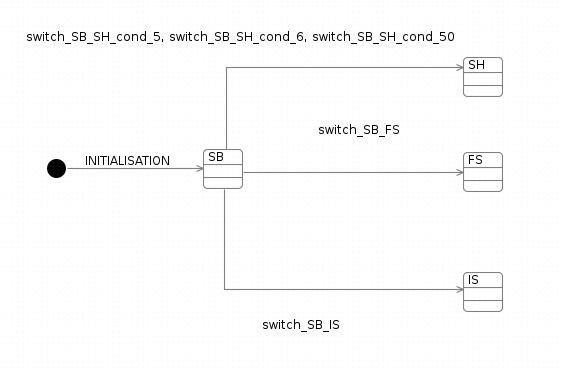
\includegraphics[width=.75\textwidth]{statechart4}
  \caption{Statemachine for Machine 3}
  \label{fig:statemachine-m3}
\end{figure}



The RBC can grant a shunting request and display the information to acknowledge
shunting. This is represented by the Boolean state variables
\bvar{shunting\_granted\_RBC} and \bvar{display\_shunting\_ack}. The driver can
isolate the ETCS system, he can manually select shunting, execute a shunting
request and acknowledge when the train switches to shunting. This is represented
by the Boolean state variables \bvar{driver\_select\_shunting},
\bvar{driver\_request\_shunting}, \bvar{driver\_ack\_shunting} and
\bvar{driver\_isolates\_ETCS}.

These variables are set as active by events representing the respective actions
by the RBC or the driver. Events which have one of these actions as precondition
will reset the events, e.g., displaying the shunting acknowledge
(\bevent{display\_shunting\_ok}) needs a previous request as precondition and
will reset the variable \bvar{driver\_request\_shunting} when it is executed.

\paragraph{Implemented Requirements}
\label{sec:impl-requ-1}

\begin{itemize}
\item §4.6.2 condition [5]
\item §4.6.2 condition [6]
\item §4.6.2 condition [10]
\item §4.6.2 condition [50]
\item priority of \bvar{SB} to \bvar{IS} over \bvar{SB} to \bvar{SH} and
  \bvar{SB} to \bvar{FS}
\end{itemize}

{\bf NOTE:} The invariant, that the preconditions of the transitions with the
same priorities are mutually exclusive, does not hold, i.e., ($[5] \vee [6] \vee
[50]) \wedge [10] \neq FALSE$. Either this is an error in the specification or
there is an underlying functional dependency which is not captured if these 3
transitions are modeled in isolation.

\begin{description}
\REFINES{m2\_train\_data}
\SEES{c1\_train}
\VARIABLES
        \begin{description}
                \Item{ driver\_select\_shunting }
                \ItemY{ driver\_request\_shunting }{}
                \ItemY{ driver\_ack\_shunting }{}
                \ItemY{ display\_shunting\_ack }{}
                \ItemY{ shunting\_granted\_RBC }{}
                \ItemY{ driver\_isolates\_ETCS }{}
                \Item{ specific\_mode\_profile }
        \end{description}
\EVENTS
        \EVT {change\_specific\_mode\_profile}
                \begin{description}
                \AnyPrm
                        \begin{description}
                        \Item{l\_flag }
                        \end{description}
                \WhereGrd
                        \begin{description}
                        \nItem{ grd1 }{ l\_flag \in  BOOL }
                        \end{description}
                \ThenAct
                        \begin{description}
                        \nItem{ act1 }{ specific\_mode\_profile :=  l\_flag }
                        \end{description}
                \EndAct
                \end{description}
        \EVT {driver\_isolates\_ETCS}
                \begin{description}
                \WhenGrd
                        \begin{description}
                        \nItem{ grd1 }{ driver\_isolates\_ETCS = FALSE }
                        \end{description}
                \ThenAct
                        \begin{description}
                        \nItem{ act1 }{ driver\_isolates\_ETCS :=  TRUE }
                        \end{description}
                \EndAct
                \end{description}
        \EVT {driver\_select\_shunting}
                \begin{description}
                \WhenGrd
                        \begin{description}
                        \nItem{ grd1 }{ current\_level \in  \{ NTC, L0, L1\}  }
                        \end{description}
                \ThenAct
                        \begin{description}
                        \nItem{ act1 }{ driver\_select\_shunting :=  TRUE }
                        \end{description}
                \EndAct
                \end{description}
        \EVT {driver\_request\_shunting}
                \begin{description}
                \WhenGrd
                        \begin{description}
                        \nItem{ grd1 }{ current\_level \in  \{ L2, L3\}  }
                        \end{description}
                \ThenAct
                        \begin{description}
                        \nItem{ act1 }{ driver\_request\_shunting :=  TRUE }
                        \end{description}
                \EndAct
                \end{description}
        \EVT {display\_shunting\_ack}\cmt{		\\\hspace*{4,6 cm}  train acknowledges shunting -$>$  specific mode required? }
                \begin{description}
                \WhenGrd
                        \begin{description}
                        \nItemY{ grd1 }{ driver\_request\_shunting = TRUE }{ }
                        \nItem{ grd2 }{ display\_shunting\_ack = FALSE }
                        \end{description}
                \ThenAct
                        \begin{description}
                        \nItemY{ act1 }{ display\_shunting\_ack :=  TRUE }{  }
                        \nItemY{ act2 }{ driver\_request\_shunting :=  FALSE }{  }
                        \nItemY{ act3 }{ shunting\_granted\_RBC :=  TRUE }{  }
                        \end{description}
                \EndAct
                \end{description}
        \EVT {driver\_ack\_shunting}
                \begin{description}
                \WhenGrd
                        \begin{description}
                        \nItem{ grd1 }{ display\_shunting\_ack = TRUE }
                        \end{description}
                \ThenAct
                        \begin{description}
                        \nItemY{ act1 }{ driver\_ack\_shunting :=  TRUE }{  }
                        \end{description}
                \EndAct
                \end{description}
        \EVT {switch\_SB\_SH\_cond\_5}
        \EXTD {switch\_SB\_SH\_cond\_5}
                \begin{description}
                \WhenGrd
                        \begin{description}
                        \nItemX{ isin\_SB }{ SB = TRUE }
                        \nItemX{ grd2 }{ current\_level \in  \{ NTC, L0, L1\}  }
                        \nItemXY{ grd1 }{ current\_behavior = standstill }{ }
                        \nItem{ grd4 }{ driver\_isolates\_ETCS = FALSE }
                        \nItemY{ grd3 }{ driver\_select\_shunting = TRUE }{ }
                        \end{description}
                \ThenAct
                        \begin{description}
                        \nItemX{ enter\_SH }{ SH :=  TRUE }
                        \nItemX{ leave\_SB }{ SB :=  FALSE }
                        \nItem{ act1 }{ driver\_select\_shunting :=  FALSE }
                        \end{description}
                \EndAct
                \end{description}
        \EVT {switch\_SB\_SH\_cond\_6}
        \EXTD {switch\_SB\_SH\_cond\_6}
                \begin{description}
                \WhenGrd
                        \begin{description}
                        \nItemX{ isin\_SB }{ SB = TRUE }
                        \nItemXY{ grd1 }{ current\_behavior = standstill }{ }
                        \nItemX{ grd2 }{ current\_level \in  \{ L2, L3\}  }
                        \nItem{ grd3 }{ driver\_isolates\_ETCS = FALSE }
                        \end{description}
                \ThenAct
                        \begin{description}
                        \nItemX{ enter\_SH }{ SH :=  TRUE }
                        \nItemX{ leave\_SB }{ SB :=  FALSE }
                        \nItem{ act1 }{ shunting\_granted\_RBC :=  FALSE }
                        \nItem{ act2 }{ display\_shunting\_ack :=  FALSE }
                        \end{description}
                \EndAct
                \end{description}
        \EVT {switch\_SB\_SH\_cond\_50}
        \EXTD {switch\_SB\_SH}
                \begin{description}
                \WhenGrd
                        \begin{description}
                        \nItemX{ isin\_SB }{ SB = TRUE }
                        \nItemY{ grd2 }{ driver\_ack\_shunting = TRUE }{ }
                        \nItemY{ grd1 }{ display\_shunting\_ack = TRUE }{ }
                        \nItem{ grd3 }{ driver\_isolates\_ETCS = FALSE }
                        \end{description}
                \ThenAct
                        \begin{description}
                        \nItemX{ enter\_SH }{ SH :=  TRUE }
                        \nItemX{ leave\_SB }{ SB :=  FALSE }
                        \nItem{ act2 }{ driver\_ack\_shunting :=  FALSE }
                        \nItemY{ act1 }{ display\_shunting\_ack :=  FALSE }{  }
                        \end{description}
                \EndAct
                \end{description}
        \EVT {switch\_SB\_FS}
        \EXTD {switch\_SB\_FS}
                \begin{description}
                \WhenGrd
                        \begin{description}
                        \nItemX{ isin\_SB }{ SB = TRUE }
                        \nItemXY{ grd1 }{ MA\_SSP\_gradient\_data = TRUE }{ }
                        \nItemX{ grd2 }{ valid\_train\_data = TRUE }
                        \nItem{ grd4 }{ specific\_mode\_profile = FALSE }
                        \nItem{ grd3 }{ driver\_isolates\_ETCS = FALSE }
                        \end{description}
                \ThenAct
                        \begin{description}
                        \nItemX{ enter\_FS }{ FS :=  TRUE }
                        \nItemX{ leave\_SB }{ SB :=  FALSE }
                        \end{description}
                \EndAct
                \end{description}
        \EVT {switch\_SB\_IS}
        \EXTD {switch\_SB\_IS}
                \begin{description}
                \WhenGrd
                        \begin{description}
                        \nItemX{ isin\_SB }{ SB = TRUE }
                        \nItem{ grd1 }{ driver\_isolates\_ETCS = TRUE }
                        \end{description}
                \ThenAct
                        \begin{description}
                        \nItemX{ enter\_IS }{ IS :=  TRUE }
                        \nItemX{ leave\_SB }{ SB :=  FALSE }
                        \nItem{ act1 }{ driver\_isolates\_ETCS :=  FALSE }
                        \end{description}
                \EndAct
                \end{description}
\END
\end{description}


\end{document}


%%% Local Variables:
%%% mode: latex
%%% TeX-master: t
%%% End:
